\documentclass[9pt]{article}

\usepackage{graphicx, xcolor, amssymb} % Required for inserting images
\usepackage{amsmath}
\usepackage{amsfonts}
\usepackage{ctex}
\usepackage{enumitem}
\usepackage{longtable}
\usepackage{makecell} % 换行

% 使用分栏宏包
\usepackage{multicol} 
\usepackage{multirow}
\setlength{\columnseprule}{0.4pt} % 分割线

% 设置字体
\usepackage{unicode-math}
\setmainfont{Cambria}
\setmathfont{Cambria Math}

% 调整页面布局
\usepackage[a4paper, top=0.7cm, bottom=1cm, left=0.7cm, right=.7cm]{geometry}
\setlength{\footskip}{15pt}

% 设置页脚/页眉
\usepackage{fancyhdr}
\fancyfoot[C]{Copyright By Jingren Zhou | Page \thepage}
\fancyhead[]{}
\pagestyle{fancy}
% 去除线
\renewcommand{\headrulewidth}{0pt}
\renewcommand{\footrulewidth}{0pt}

% 设置 section/subsection 之间的行间距
\usepackage{titlesec}
\titlespacing*{\section}{0pt}{0pt}{0pt}
\titlespacing*{\subsection}{0pt}{0pt}{0pt}

% 调整标题上下间距
\usepackage{titling}
\setlength{\droptitle}{-2.4cm} % 负值表示向上移动

% 设置标题,作者,时间
\title{LPMS Note}
\author{}
\date{}

% 正文
\begin{document}


% 标题
\maketitle
\thispagestyle{fancy}
\vspace{-3.5cm}

% 字体大小
\fontsize{10pt}{11pt}\selectfont
\setlength{\parindent}{8pt}


\section{General LP} % General Linear Programming Problem

\textbf{General LP Problem}: {\small \textbf{Decision Variables}: $x_i$ \quad \textbf{parameters}: $a_{ij},b_i,c_i$ \quad \textbf{Objective Function}: $f$ \quad \textbf{Constraints}: {\small subject to 后边的部分}}

\vspace{-9pt}
\begin{multicols}{2}

    LP problem can be written as:
    \[
    \begin{aligned}
        \text{maximize} \quad \ \ f = & c_1x_1 + c_2x_2 + \cdots + c_nx_n & \\
        \text{subject to} \quad \qquad & a_{11}x_1 + a_{12}x_2 + \cdots + a_{1n}x_n \leq b_1 & \\
                                & a_{21}x_1 + a_{22}x_2 + \cdots + a_{2n}x_n \leq b_2 & \\
                                & \vdots & \\
                                & a_{m1}x_1 + a_{m2}x_2 + \cdots + a_{mn}x_n \leq b_m & \\
                                & x_1 \geq 0, x_2 \geq 0, \cdots, x_n \geq 0 &
    \end{aligned}
    \]
    
    \columnbreak

    We can also write the LP problem in matrix form:

    \vspace{5pt}
    $
    A=
    \begin{pmatrix}
        a_{11} & \cdots & a_{1n} \\
        \vdots & \ddots & \vdots \\
        a_{m1} & \cdots & a_{mn} \\
    \end{pmatrix}
    ,\mathbf{b}=
    \begin{pmatrix}
        b_1 \\
        \vdots \\
        b_m
    \end{pmatrix}
    ,\mathbf{c}=
    \begin{pmatrix}
        c_1 \\
        \vdots \\
        c_n
    \end{pmatrix}
    ,\mathbf{x}=
    \begin{pmatrix}
        x_1 \\
        \vdots \\
        x_n
    \end{pmatrix}
    $

    \[
    \begin{aligned}
        \text{maximize} \quad \ \ f = & \mathbf{c}^T\mathbf{x} & \\
        \text{subject to} \quad \qquad & A\mathbf{x} \leq \mathbf{b} & \mathbf{x} \geq 0 \\
    \end{aligned}
    \]
\end{multicols}

\vspace{-15pt}
\textbf{Feasible Solution}: If $\mathbf{x}$ satisfies all constraints (i.e. $A\mathbf{x}\leq\mathbf{b}$), then $\mathbf{x}$ is a feasible solution. {\footnotesize (可行解)}\quad \textbf{Optimal Sol}: {\footnotesize (最优解) (可多个)}

\textbf{Find Optimal Solution}: \textbf{Graphical Method}: {\footnotesize 略.} \quad \textbf{Vertex Enumeration}: {\footnotesize 所有顶点检查, 找出最优解.} \quad \textbf{Simplex Method}: {\footnotesize 后面详述.}

\textbf{Slack Variables}: For each inequality constraint, we introduce a slack variable $x_i$ ($i>n$) to convert it to an equation. {\footnotesize (松弛变量)}

\vspace{-9pt}
\begin{multicols}{2}

    LP problem can be written as: \quad \quad ps: $x_{i}\geq0$ ($i>n$).
    \[
    \begin{aligned}
        \text{maximize} \quad \ \ f = & c_1x_1 + c_2x_2 + \cdots + c_nx_n & \\
        \text{subject to} \quad \qquad & a_{11}x_1 + a_{12}x_2 + \cdots + a_{1n}x_n + x_{n+1} = b_1 & \\
                                & a_{21}x_1 + a_{22}x_2 + \cdots + a_{2n}x_n + x_{n+2} = b_2 & \\
                                & \vdots & \\
                                & a_{m1}x_1 + a_{m2}x_2 + \cdots + a_{mn}x_n + x_{n+m} = b_m & \\
                                & x_1 \geq 0, x_2 \geq 0, \cdots, x_{n+m} \geq 0 &
    \end{aligned}
    \]
    
    \columnbreak

    We can also write the LP problem in matrix form:

    \vspace{5pt}
    $
    \overline{A}= [ \ A  \ \ I_m \ ]
    ,\mathbf{b}=\mathbf{b}
    ,\overline{\mathbf{c}}=
    \begin{pmatrix}
        \mathbf{c} \\
        \mathbf{0}_{ m\times 1}
    \end{pmatrix}
    ,\mathbf{x}=
    \begin{pmatrix}
        \mathbf{x} \\
        \vdots \\
        x_{n+m}
    \end{pmatrix}
    $

    \[
    \begin{aligned}
        \text{maximize} \quad \ \ f = & \overline{\mathbf{c}}^T\mathbf{x} & \\
        \text{subject to} \quad \qquad & \overline{A}\mathbf{x} = \mathbf{b} & \mathbf{x} \geq 0 \\
    \end{aligned}
    \]

    \vspace{-20pt}
    \textbf{Solving}: $\mathbf{x}=\mathbf{x}_b+\mathbf{v}$ where $\overline{A}\mathbf{v}=0$ and $\mathbf{x}_b=[\mathbf{0} \ \mathbf{b}]^T$

\end{multicols}

\vspace{-15pt}
\textbf{Feasible Region}: {\small It's the set $K$ of the solutions to $\overline{A}\mathbf{x}=\mathbf{b}$} \quad \textbf{Convex Set}: {\small The set $K$ is convex if $\forall \mathbf{x},\mathbf{x'}\in K$, $\forall\theta\in[0,1],\mathbf{x}_{\theta}=(1-\theta)\mathbf{x}+\theta\mathbf{x'}\in K$.}

\textbf{Vertex on Convex Set}: {\footnotesize A vertex of the convex set $K$ is a point $\mathbf{x}\in K$ which doesn't lie strictly inside any line segment connecting two points in $K$.}

$\cdot$ \textbf{Theorem}: {\small If LP has a unique optimal solution is a vertex.} \quad \quad \textbf{Theorem}: {\small If LP has a non-unique solution, $\exists$ optimal solution at vertex}


\section{Simplex Method} % Simplex Method

\subsection{Simplex Algorithm}

\textbf{Solve LP Problem}: Assume $f=\overline{\mathbf{c}}^T\mathbf{x}$ with $\overline{A}\mathbf{x}=\mathbf{b}$ and $\mathbf{x}\geq0$.

\begin{enumerate}[itemsep=-2pt, topsep=-2pt]
    \item {\footnotesize 修改$x_i$/列顺序,$A$中换顺序后得到可逆的$B_{m\times m}$ \ \ $\Rightarrow$ \ \ $\overline{A}\mathbf{x}=\mathbf{b}\Leftrightarrow B\mathbf{x}_B+N\mathbf{x}_N=\mathbf{b}$ \quad $\overline{\mathbf{c}}\rightarrow[\mathbf{c}_B \ \mathbf{c}_N]^T$ \ \ $\overline{A}\rightarrow[B \ N]$ \ \ $\mathbf{x}\to[\mathbf{x}_B \ \mathbf{x}_N]^T$ \quad Let $\widehat{\mathbf{b}}=B^{-1}\mathbf{b}$ \ \ $\widehat{N}=B^{-1}N$}
    \item \textbf{Solution}: $\mathbf{x}_B=\widehat{\mathbf{b}}-\widehat{N}\mathbf{x}_N$ \quad \quad If $\mathbf{x}_N=0$ $\Rightarrow$ It's a basic solution. {\scriptsize (But we need to check whether $\mathbf{x}_B\geq0$)} \quad \quad {\scriptsize Using $\mathcal{B},\mathcal{N}$: Index set of independent/else.}
    \item \textbf{Basic Variables}: $\mathbf{x}_B$ \quad \textbf{Nonbasic Variables}: $\mathbf{x}_N$
    \item \textbf{At Basic Solution}: $\mathbf{x}_B=\widehat{\mathbf{b}},\mathbf{x}_N=\mathbf{0}$ \quad $\Rightarrow$ \quad If $\widehat{\mathbf{b}}\geq0$. Corresponding $\mathbf{x}$ is: $^1$ vertex of $K$; \ \ $^2$ \textbf{Basic Feasible Solution (BFS)}
    \item \textbf{Basic Costs}: $\mathbf{c}^T_B$ \quad \textbf{Nonbasic Costs}:$\mathbf{c}^T_N$ \quad \textbf{Reduced Costs}: $\widehat{\mathbf{c}}_N=\mathbf{c}_N -\widehat{N}^T\mathbf{c}_B=\mathbf{c}_N-N^TB^{-T}\mathbf{c}_B$ \quad $\widehat{f}=\mathbf{c}_B^T\widehat{\mathbf{b}}$ \quad \quad $\mathbf{x}_B,\mathbf{x}_N\geq0$
    \item \textbf{Objective Value}: $f=\overline{\mathbf{c}}^T\mathbf{x}=\mathbf{c}^T_B\mathbf{x}_B+\mathbf{c}^T_N\mathbf{x}_N=\widehat{f}+\widehat{\mathbf{c}}_N^T\mathbf{x}_N$ \quad \quad If $\widehat{\mathbf{c}}_N\leq0$, then $f\leq\widehat{f}$ \ \ $\Rightarrow$ \ \ Corresponding $\mathbf{x}$ is optimal.
    \item If $\widehat{\mathbf{c}}_N\leq0$ doesn't hold, we using \textbf{Simplex Algorithm}.
\end{enumerate}

\textbf{Simplex Algorithm}:

\begin{enumerate}[itemsep=-2pt, topsep=-2pt]
    \item {\small \textbf{Initial Basic Feasible Solution}: Try $\mathcal{B}=\{n+1,...,n+m\}$ and $\mathcal{N}=\{1,...,n\}$ \ \ $\Rightarrow$ \ \ $B=I,N=A$ , $\mathbf{x}_B=\widehat{\mathbf{b}}=\mathbf{b}$, $\mathbf{x}_N=\mathbf{0}$, $\mathbf{c}_B=\mathbf{0}$, $\mathbf{c}_N=\mathbf{c}$}
    \item If $\mathbf{b}\geq0$. $\Rightarrow$ Basis is feasible + cont. \qquad Else: Basis $B$ is not feasible. \quad Go to ``Cases If $\mathbf{b}\ngeq0$``
    \item If $\widehat{\mathbf{c}}_N\leq0. \Rightarrow$ Optimal Solution \qquad Else: cont.
    \item Let $q'\in\mathcal{N}$ {\small 对应$\widehat{\mathbf{c}}_N$中最大positive分量的index} \quad {\small 同理,对应的最大正分量值为$\widehat{c_q}$} \quad {\small 对应的variable为$x_{q'}$} \quad {\small 对应$N$中的[$q$]列为$\mathbf{a}_q$}
    \item Let $\widehat{\mathbf{a}_q}=B^{-1}\mathbf{a_q}$. \qquad If $\widehat{\mathbf{a}_q}\leq0$ $\Rightarrow$ LP is unbounded. \qquad Else: LP is bounded + cont.
    \item Let $p'\in\mathcal{B}$ \ be the index corresponding to $p=\arg\min_{i=1,...,m \ ; \ \widehat{a}_{iq}>0}\frac{\widehat{b_i}}{\widehat{a}_{iq}}$ {\scriptsize $p$是对应的index,not value} \qquad \quad {\small 用$\overline{\alpha}=\frac{\widehat{b_p}}{\widehat{a}_{pq}}$代表值}\\
    $\widehat{b_i},\widehat{a}_{iq}$ {\small 代表$\widehat{\mathbf{b}}$的第$i$个分量, $\widehat{\mathbf{a}_q}$的第$i$个分量} \\
    {\small $p'$代表能使$\frac{\widehat{b_i}}{\widehat{a}_{iq}}$的值最小的index,前提条件是$\widehat{a}_{iq}>0$} \qquad \qquad {对应的variable为$x_{p'}$}
    \item Exchange $p'$ and $q'$ between $\mathcal{B}$ and $\mathcal{N}$ \ \ $\Rightarrow$ \qquad Update $\mathcal{B},\mathcal{N},B,N,\widehat{\mathbf{b}},...$ \quad {\scriptsize ps: New $B := B + (a_q - B e_p) e_p^T$}
    \item Go to 3.
\end{enumerate}


\textbf{Case: If $\mathbf{b}\ngeq0$}: \textbf{Phase I Problem}
\begin{enumerate}[itemsep=-2pt, topsep=-2pt]
    \item Subtract \textbf{artificial variables} $x_{n+m+1},...,x_{n+m+m}\geq0$ and change objective function $f$ to: \\    
    {\centering 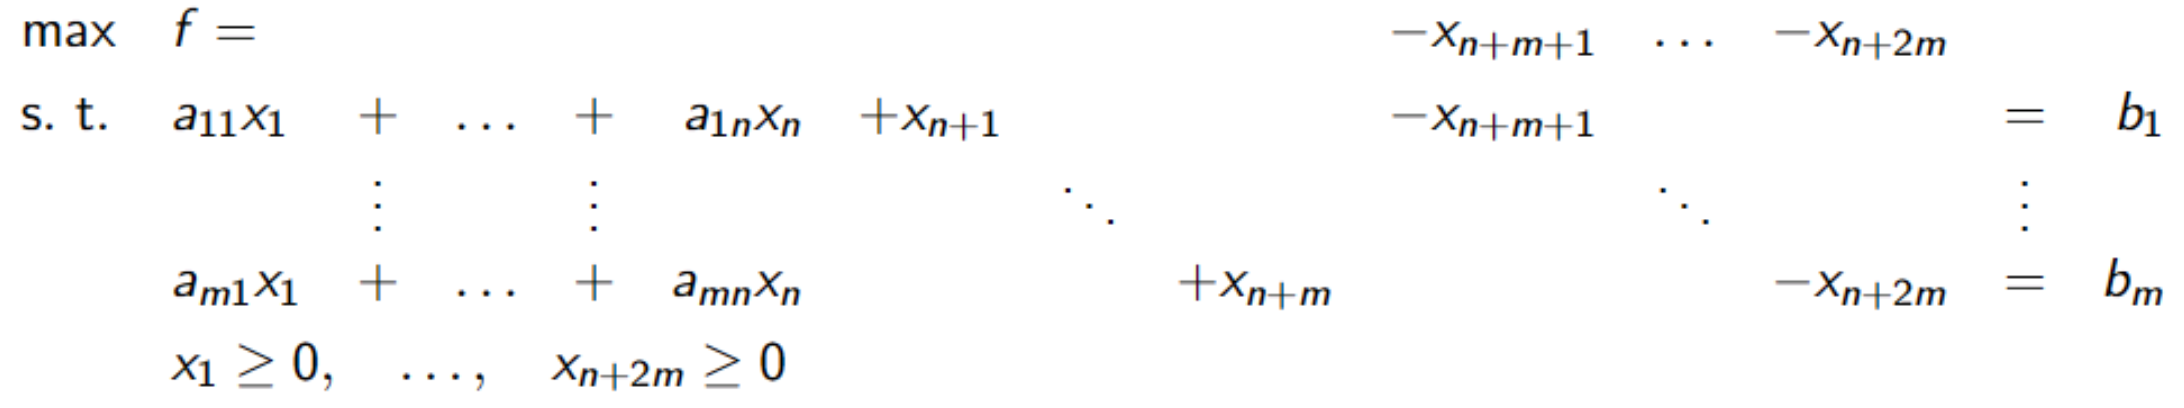
\includegraphics[width=0.6\textwidth]{formula.png}}
    \item Let {\small Basic Variables: $\mathbf{x}_{B}=$ 第i个元素是: $x_{n+i}=b_i$ (if $b_i\geq0$) \quad 是:$x_{n+m+i}=-b_i$ (if $b_i<0$) $\star$} \\
    {\small Let Nonbasic Variables: $\mathbf{x}_{N}=$ 第i个元素是: $x_{n+m+i}=0$ (if $b_i\geq0$)} \quad  是:$x_{n+i}=b_i$ (if $b_i<0$)\\
    {\small Let Basic Matrix $B=$ 第i列是: $\mathbf{e}_i$ (if $b_i\geq0$) 否则: $-\mathbf{e}_i$ 其他列是$N$的对应列 \qquad \quad Let $\widehat{\mathbf{b}}=B^{-1}\mathbf{b}=|\mathbf{b}|\geq0$} \\
    {\small Let $\mathbf{c}_B=$ $x_B$对应的$f$中的系数  \qquad $\mathbf{c}_N=$同理 \qquad $\widehat{\mathbf{c}}_N=\mathbf{c}_N-N^TB^{-T}\mathbf{c}_B$}
    \item \textbf{Size of Infeasibility}: is $\sum^m_{i=1}x_{n+m+i}$ \qquad $f=-\sum^m_{i=1}x_{n+m+i}\leq0$
    \item If $f=0$, $\mathbf{x}$ is a BFS. $\Rightarrow$ Go to \textbf{Phase II Problem}{\small (恢复到之前的$f$并删除artificial variables)} \\
    Else: Go to \textbf{Simplex Algorithm} {\small 得到辅助问题Phase I的最优解.} \quad \textbf{If $f<0$}: LP is infeasible. \quad \textbf{If $f=0$}: LP is feasible. $\Rightarrow$ \textbf{Phase II}
\end{enumerate}

\textbf{Case: If $\mathbf{b}\ngeq0$}: \textbf{Phase II Problem}


\subsection{More thing about Simplex Algorithm}

\textbf{Degeneracy}: If $\widehat{\mathbf{b}}$ has any zero component, then $\mathbf{x}$ is a \textbf{degenerate vertex}. \qquad {\scriptsize 如果$\widehat{\mathbf{b}}$的第$p$个分量$\widehat{\mathbf{b}}_p=0$,那么单纯形法可能会陷入循环.}

\quad \textbf{Theorem}: If no degenerate situation, then Simplex Algorithm will terminate in a finite number of steps.

\textbf{Examples}: 1.The worst case of Simplex Algorithm. \ \ 2. Cyclic case of Simplex Algorithm.

\begin{enumerate}[itemsep=-2pt, topsep=-2pt]
    \item \textbf{Klee-Minty Problem}: max $f=\sum^n_{j=1}10^{j-1}x_j$ \quad ; \quad s.t. $x_i+2\sum^n_{j=i+1}10^{j-i}x_j\leq100^{n-i}$ for $i=1,...,n$ \quad ; \quad $x_i\geq0$ \\
    has $2^n$ vertices. \quad \textbf{Worst Case}: $2^n-1$ iterations.
    \item \textbf{Hall-McKinnon Problem}: max $f=x_1-5.5x_2+0.75x_3-5.75x_4$ \quad ; \quad {\scriptsize s.t.} {\tiny $2.5x-19.5x_2-3.5x_3+19.5x_4+x_5=0$ ; $0.5x_1-3.5x_2-0.5x_3+3.5x_4+x_6=0$ ; $x_i\geq0$}
\end{enumerate}


\subsection{Sparsity LP Problem}

\textbf{Implementation}: 计算/编程中的计算化简 \qquad Consider: $\widehat{\mathbf{b}}=B^{-1}\mathbf{b}$ \ \ $\widehat{\mathbf{c}}_N=\mathbf{c}_N-N^TB^{-T}\mathbf{c}_B$ \ \ $\widehat{\mathbf{a}}_q=B^{-1}\mathbf{a}_q$

\begin{enumerate}[itemsep=-2pt, topsep=-2pt]
    \item Solve: \( B \hat{b} = b \) \quad to get: \(\hat{b} = B^{-1}b\)
    \item Solve: \( B^T \pi = c_B \) \quad to get: \(\pi = B^{-T}c_B\)
    \item Solve: \(\hat{c}_N = c_N - N^T\pi\) \quad to get: \(\hat{c}_N = c_N - N^TB^{-T}c_B\)
    \item Solve: \( B^T \hat{a}_q = a_q \) \quad to get: \(\hat{a}_q = B^{-T}a_q\)
    \item Matrix $B$ is \textbf{sparse} and \textbf{invertible}. And in Simplex Algorithm, the next matrix $B$ obtained by $B := B + (a_q - B e_p) e_p^T$
\end{enumerate}

\textbf{Sparse LP Problem}: For LP problem: max $f=\mathbf{c}^T\mathbf{x}$ \quad s.t. $A\mathbf{x}=\mathbf{b}$ \quad $\mathbf{x}\geq0$

\qquad It is \textbf{sparse} if the matrix $A$ is sparse. (i.e. Most of the elements of $A$ are zero)

\textbf{Find Inverse of $B$}: Use \textbf{Guassian Elimination} to decomposition $B$ into $LU$ where $L$ is lower triangular and $U$ is upper triangular.

\quad Then we can solve $B\mathbf{x}=\mathbf{b}$ by solving $^1$ $L\mathbf{y}=\mathbf{b}$ and $^2$ $U\mathbf{x}=\mathbf{y}$

\vspace{-5pt}
{\scriptsize 
\[
\begin{bmatrix}
a_{11} & a_{12} & a_{13} & a_{14} \\
a_{21} & a_{22} & a_{23} & a_{24} \\
a_{31} & a_{32} & a_{33} & a_{34} \\
a_{41} & a_{42} & a_{43} & a_{44} 
\end{bmatrix}
=
\begin{bmatrix}
1 & 0 & 0 & 0 \\
l_{21} & 1 & 0 & 0 \\
l_{31} & l_{32} & 1 & 0 \\
l_{41} & l_{42} & l_{43} & 1
\end{bmatrix}
\begin{bmatrix}
u_{11} & u_{12} & u_{13} & u_{14} \\
0 & u_{22} & u_{23} & u_{24} \\
0 & 0 & u_{33} & u_{34} \\
0 & 0 & 0 & u_{44}
\end{bmatrix}
=
\begin{bmatrix}
\textcolor{red}{u_{11}} & \textcolor{red}{u_{12}} & \textcolor{red}{u_{13}} & \textcolor{red}{u_{14}} \\
\textcolor{orange}{l_{21} u_{11}} & \textcolor{olive}{l_{21} u_{12} + u_{22}} & \textcolor{olive}{l_{21} u_{13} + u_{23}} & \textcolor{olive}{l_{21} u_{14} + u_{24}} \\
\textcolor{orange}{l_{31} u_{11}} & \textcolor{green}{l_{31} u_{12} + l_{32} u_{22}} & \textcolor{blue}{l_{31} u_{13} + l_{32} u_{23} + u_{33}} & \textcolor{blue}{l_{31} u_{14} + l_{32} u_{24} + u_{34}} \\
\textcolor{orange}{l_{41} u_{11}} & \textcolor{green}{l_{41} u_{12} + l_{42} u_{22}} & \textcolor{black}{l_{41} u_{13} + l_{42} u_{23} + l_{43} u_{33}} & \textcolor{purple}{l_{41} u_{14} + l_{42} u_{24} + l_{43} u_{34} + u_{44}}
\end{bmatrix}
\]
}
\vspace{-5pt}

\quad By Solving $\textcolor{red}{\blacksquare} \to \textcolor{orange}{\blacksquare} \to \textcolor{olive}{\blacksquare} \to \textcolor{green}{\blacksquare} \to \textcolor{blue}{\blacksquare} \to \textcolor{black}{\blacksquare} \to \textcolor{purple}{\blacksquare}  $


\section{Sensitive Analysis} % Sensitive Analysis

\textbf{RHS Sensitivity}: {\small Consider $b_i\to b_i+\delta$ \quad $\big|$ \quad $\max f=\mathbf{c}^T\mathbf{x}$ subject to $A\mathbf{x}\leq \mathbf{b},\mathbf{x}\geq0$ \quad $\Rightarrow$ {\tiny (Add Slack variables)} \quad $\max f=\overline{\mathbf{c}}^T\mathbf{x}$ subject to $\overline{A}\mathbf{x}=\mathbf{b},\mathbf{x}\geq0$}

\qquad Assume $\mathcal{B},\mathcal{N},B,N$ yield an \textit{optimal solution}, with $\mathbf{x}_B=\widehat{\mathbf{b}},\mathbf{x}_N=\mathbf{0}$

\qquad Then, the new optimal values is: \quad $\mathbf{x}_B=B^{-1}(\mathbf{b}+\delta \mathbf{e}_i)=\widehat{\mathbf{b}}+\delta B^{-1}\mathbf{e_i}$ \quad if $\mathbf{x}_B\geq0$

\qquad With range of $\delta\in[ \ \underline{\delta} \ , \ \overline{\delta} \ ]$ \quad $\underline{\delta}=\max\limits_{[B^{-1}]_{ij}>0}-\frac{\widehat{b}_j}{[B^{-1}]_{ij}}$ \quad $\overline{\delta}=\min\limits_{[B^{-1}]_{ij}<0}-\frac{\widehat{b}_j}{[B^{-1}]_{ij}}$ \hspace{30pt} {\tiny $\Downarrow \text{nonbasic slack}:\pi_i=-\widehat{c_i}$, $\widehat{c_i}$ 指 reduced cost $\widehat{\mathbf{c}}_N$ 的第$i$个分量;basic slack: $\pi_i=0$}

\qquad \textbf{Fair Prices}: The objective function will change by $\delta$ as: $f=\widehat{f}+\delta\pi_i$ \quad where $\widehat{f}=\mathbf{c}_B^T\widehat{\mathbf{b}}$ \quad $\pi_i=\mathbf{c}_B^TB^{-1}\mathbf{e}_i$ (fair price)

\qquad If \textit{price of unit amount} $<$ $\pi_i$, buying more of the resource is attractive. \qquad If $>$, is unattractive.

\qquad ps: 如果$b_i\to b_i+\delta$ 对应的$\mathcal{B}$中的第$i$个变量是basic slack, 那么$\pi_i=0$. (simply no fair price price for more of the resource)

\qquad ps: 如果$b_i\to b_i+\delta$ 对应的$\mathcal{B}$中的第$i$个变量不是slack, {\tiny (Same as $x_{n+i}$ is nonbasic slack)}, 那么$\pi_i=-\widehat{c_i}$.

\qquad $\star$ Range of $\delta$ is \textit{lower|upper bound Sensitivity}, \quad $\star$ \textit{Feasible Region} increases when $\overline{\delta}$ increases and $\underline{\delta}$ decreases.

\textbf{Cost Sensitivity}: 即$c_i\to c_i+\delta$. \quad $\max f=\mathbf{c}^T\mathbf{x}$ subject to $A\mathbf{x}\leq \mathbf{b},\mathbf{x}\geq0$

\begin{enumerate}[itemsep=-2pt, topsep=-2pt]
    \item 小范围的变化不会改变最优解. {\scriptsize (If an LP cost coefficient is changed by a small amount, the optimal solution will not change.)}
    \item 如果$c_i\to c_i+\delta$ 对应的$i$变量在$\mathcal{B}$中(basic variables), 那么 all reduced costs will change.
    \item 如果$c_i\to c_i+\delta$ 对应的$i$变量在$\mathcal{N}$中(nonbasic variables), 那么 only the reduced cost of \textit{that} variables will change.
\end{enumerate}

\textbf{Coefficient Sensitivity}: 即$a_{ij}\to a_{ij}+\delta$. \quad $\max f=\mathbf{c}^T\mathbf{x}$ subject to $A\mathbf{x}\leq \mathbf{b},\mathbf{x}\geq0$

\begin{enumerate}[itemsep=-2pt, topsep=-2pt]
    \item 如果影响的变量在$\mathcal{B}$中(basic variables): $B$ may become singular, the optimal solution may change, etc.
    \item 如果影响的变量在$\mathcal{N}$中(nonbasic variables): One \textit{reduced cost} will change, $N$ will change.
\end{enumerate}


\section{Duality} % Duality

\textbf{Duality}: For LP problem: max $f=\mathbf{c}^T\mathbf{x}$ \quad s.t. $A\mathbf{x}\leq \mathbf{b}, \quad\mathbf{x}\geq0$ \quad \textbf{Primal} problem \qquad $(P)$

\qquad \ \ The \textbf{dual} problem is: min $f=\mathbf{b}^T\mathbf{y}$ \quad s.t. $A^T\mathbf{y}\geq \mathbf{c}, \quad\mathbf{y}\geq0$ \quad \textbf{Dual} problem \qquad $(D)$

\qquad \ \ - It is \textit{equivalence} to: max $f=-\mathbf{b}^T\mathbf{y}$ \quad s.t. $-A^T\mathbf{y}\leq -\mathbf{c}, \quad\mathbf{y}\geq0$

\qquad \ \ The \textbf{dual} of $(D)$ is: min $f=-\mathbf{c}^T\mathbf{z}$ \quad s.t. $(-A^T)^T\mathbf{z}\geq (-\mathbf{b}), \ \ (\text{i.e.} \ -A\mathbf{z}\geq -\mathbf{b})$, $\quad\mathbf{z}\geq0$

\qquad \ \ - It is \textit{equivalence} to: max $f=\mathbf{c}^T\mathbf{z}$ \quad s.t. $A\mathbf{z}\leq \mathbf{b}, \quad\mathbf{z}\geq0$, which is the \textbf{Primal} problem $(P)$.

\textbf{Weak Duality Theorem}: If $\mathbf{x}$ is feasible for $(P)$ and $\mathbf{y}$ is feasible for $(D)$, then $\mathbf{c}^T\mathbf{x}\leq\mathbf{b}^T\mathbf{y}$.

\quad \textbf{Corollary}: {\footnotesize If $\mathbf{x}$ for $(P)$ and $\mathbf{y}$ for $(D)$}, then: \qquad If $(P)$ is unbounded \ \ $\Rightarrow$ \ \ $(D)$ is infeasible. \qquad If $(D)$ is unbounded \ \ $\Rightarrow$ \ \ $(P)$ is infeasible.

\textbf{Strong Duality Theorem}: If $\mathbf{x}^*$ is optimal (basic) solution for $(P)$, then:

\qquad $\mathbf{y}^*=\pi=B^{-T}\mathbf{c}_B$ is optimal solution for $(D)$, \quad and $\mathbf{c}^T\mathbf{x}^*=\mathbf{b}^T\mathbf{y}^*$.

\textbf{Application}: If LP problem: max $f=\mathbf{c}^T\mathbf{x}$ \quad s.t. $A\mathbf{x}\leq \mathbf{b}, \quad\mathbf{x}\geq0$ \quad $(P)$

\qquad is changed to a \textbf{tightening} LP problem: max $f=\mathbf{c}^T\mathbf{x}$ \quad s.t. $\begin{bmatrix} A \\ \mathbf{a}^T \end{bmatrix}\mathbf{x}\leq\begin{bmatrix}\mathbf{b} \\ b\end{bmatrix}$, $\quad\mathbf{x}\geq0$ \quad $(P')$

\qquad Then, the \textbf{relaxation dual} problem is: min $f=\mathbf{b}^T\mathbf{y}+by$ \quad s.t. $A^T\mathbf{y}+\mathbf{a}y\geq \mathbf{c}, \quad\mathbf{y}\geq0, \quad y\geq0$ \quad $(D')$

\qquad - It is \textit{equivalence} to: max $f=-\mathbf{b}^T\mathbf{y}-by$ \quad s.t. $-A^T\mathbf{y}-\mathbf{a}y\leq -\mathbf{c}, \quad\mathbf{y}\geq0, \quad y\geq0$

\qquad 此时,计算$(P')$的最优解可以通过计算$(D')$的最优解来得到. {\footnotesize (通过 \textbf{dual simplex method} 计算或equivalence to 一般的计算)}


\section{Example of format written in LP}

\textbf{Example|构建LP问题模板}:

\vspace{-10pt}
\begin{multicols}{2}
\begin{quote}
    \color{gray}
    \fontsize{7pt}{4pt}\selectfont
    \textbf{Defining decision variables}:

    \quad Let $x_1$ be the number of 1kg packets of Breakfast Blend made each day.

    \quad Let $x_2$ be the number of 1kg packets of Dinner Blend made each day.
    
    \textbf{Total income is}: $f_I = 1.16x_1 + 1.42x_2.$

    \textbf{Total cost is}: $f_C = 0.18x_1 + 0.36x_2 + 0.28x_1 + 0.16x_2 = 0.46x_1 + 0.52x_2.$

    \textbf{Thus, total profit is}:$f_I - f_C = 1.16x_1 + 1.42x_2 - 0.46x_1 - 0.52x_2 = 0.7x_1 + 0.9x_2.$

    \textbf{The objective is to maximize total profit \( f = 0.7x_1 + 0.9x_2 \)}

    \textbf{Constraints}:
    \begin{enumerate}[itemsep=-1pt, topsep=-1pt]
        \item The number of kilos of arabica used, \( 0.3x_1 + 0.6x_2 \), must not exceed the supply of 1200kg.
        \item The number of kilos of robusta used, \( 0.7x_1 + 0.4x_2 \), must not exceed the supply of 1500kg.
        \item The total number of kilos of coffee made, \( x_1 + x_2 \), must not exceed the capacity of 2400kg.
    \end{enumerate}
    
    \textbf{Thus, the LP Problem to be solved is}:
    \[
    \begin{aligned}
        \text{maximize} \qquad \ \ \ f = 0.7x_1 + 0.9x_2, \\
        \text{subject to} \quad 0.3x_1 + 0.6x_2 \leq 1200, \\
        0.7x_1 + 0.4x_2 \leq 1500, \\
        x_1 + x_2 \leq 2400, \\
        x_1, x_2 \geq 0.
    \end{aligned}
    \]
    
    \textbf{Introducing Slack Variables}:  
    \[
    \begin{aligned}
        \text{maximize} \qquad \qquad \quad f = 0.7x_1 + 0.9x_2, \\
        \text{subject to} \quad 0.3x_1 + 0.6x_2 + x_3 = 1200, \\
        0.7x_1 + 0.4x_2 + x_4 = 1500, \\
        x_1 + x_2 + x_5 = 2400, \\
        x_1, x_2, x_3, x_4, x_5 \geq 0.
    \end{aligned}
    \]
\end{quote}
\end{multicols}
\vspace{-10pt}


\textbf{Example|Iteration in Simplex Method|No Phase I,II}:

\vspace{-10pt}
\begin{quote}
    \color{gray}
    \fontsize{7pt}{4pt}\selectfont
    The RHS \( \mathbf{b} = \begin{bmatrix} 100\\ 1\end{bmatrix}\) is positive, so the ``all-slack'' basis \( \mathcal{B}=\{3,4\} \) and \(\mathcal{N}=\{1,2\}\) yields a basic feasible solution. \\
    \textbf{Iteration 1}:
    \begin{itemize}[itemsep=-1pt, topsep=-1pt]
        \item For \( \mathcal{B}=\{3,4\} \) and \( \mathcal{N}=\{1,2\} \), \(B= I\), \(N=\begin{bmatrix} 1 & 20 \\ 0 & 1\end{bmatrix}\), \( \mathbf{c}_B=\mathbf{0} \) and \( \mathbf{c}_N=\begin{bmatrix} 1 \\ 10\end{bmatrix}\), \\
        giving \( \widehat{\mathbf{b}}=B^{-1}\mathbf{b}=\begin{bmatrix} 100 \\ 1\end{bmatrix} \), and \( \widehat{\mathbf{c}}_N=\mathbf{c}_N-N^TB^{-T}\mathbf{c}_B=\begin{bmatrix} 1 \\ 10\end{bmatrix} \).
        \item Choose \(q=2\) since \( \widehat{c}_q= 10 \), and hence \( q'=2 \)
        \item Thus \(\mathbf{a}_q=\begin{bmatrix}20 \\ 0\end{bmatrix}\). Form \( \widehat{\mathbf{a}}_q=B^{-1}\mathbf{a}_q=\begin{bmatrix} 20 \\ 1\end{bmatrix} \). Since \( \widehat{\mathbf{a}}_q \) is positive, the LP is bounded.
        \item Choose \(p=\text{argmin}\left\{ \begin{matrix}\frac{100}{20} \\ (i=1)\end{matrix}, \begin{matrix}\frac{1}{1} \\ (i=2)\end{matrix}  \right\}=2 \) and hence \( p'=4 \)
    \end{itemize}
    \textbf{Iteration 2}: \(\cdots\)
    \textbf{Iteration 4}: 第一行一样, + \(\cdots\) Since \( \widehat{\mathbf{c}}_N \leq 0 \), the optimal solution is \( \mathbf{x}=\cdots \), where values of \( x_i,... = 0\) since \(\mathcal{N} = ...\)
\end{quote}
\vspace{-10pt}


\section{Additional Definition/Theorem}:

\textbf{Definition of a Convex Set}: The set $K$ is convex if, for any two points $\mathbf{x},\mathbf{x'}\in K$, the line segment $\mathbf{x}_\theta=\theta\mathbf{x}+(1-\theta)\mathbf{x'}$ for $\theta\in[0,1]$ is also in $K$.

\textbf{Definition of a Vertex of a Convex Set}: A vertex of a convex set $K$ is a point $\mathbf{x}\in K$ such that it does not lie strictly within any line segment joining two points in $K$.

\end{document}